% Chapter 2
% \ref{Chapter1}
%\begin{figure}
\chapter{Image Registration} % Main chapter title
\label{Chapter3} % For referencing the chapter elsewhere, use
%----------------------------------------------------------------------------------------

\section{Flow Chart}
\nopagebreak
% Define block styles
\tikzset{
	desicion/.style={
		diamond,
		draw,
		text width=6em,
		text badly centered,
		inner sep=0pt
	},
	block/.style={
		rectangle,
		draw,
		text width=15em,
		text centered,
		rounded corners
	},
	cloud/.style={
		draw,
		ellipse,
		minimum height=1em
	},
	descr/.style={
		fill=white,
		inner sep=2.5pt
	},
	connector/.style={
		-latex,
		font=\scriptsize
	},
	rectangle connector/.style={
		connector,
		to path={(\tikztostart) -- ++(#1,0pt) \tikztonodes |- (\tikztotarget) },
		pos=0.5
	},
	rectangle connector/.default=-2cm,
	straight connector/.style={
		connector,
		to path=--(\tikztotarget) \tikztonodes
	}
}
\begin{center}
	\begin{figure}[hbt]
		\centering
	\begin{tikzpicture}
\matrix (m)[matrix of nodes, column  sep=2cm,row  sep=8mm, align=center, nodes={rectangle,draw, anchor=center} ]{
	|[block]| {Start}              &  \\
	|[block]| { Extract the reference document to be registered from the image}               &                                            \\
	|[block]| {Compute ORB Features in the reference document \\ and scanned image}          &  \\
	|[block]| {Filter out atleast 500 matching features based on Ratio Test and Symmetry Test}    &                                             \\
	|[block]| {Find the 4 best matching features using RANSAC}    &                                          \\
	|[block]| {Compute the perspective transform that associates 4 best matching features in the reference document \\ and scanned image}    &    |[block]| {Stop}                                          \\
	|[block]| {Warp the scanned image to align it with the reference document and do bilinear interpolation}        &       |[block]| {Adaptive Thresholding}                                      \\
	|[block]| {Extract filled text from the scanned document by doing\\ background subtraction}    &   |[block]| { Add the extracted text to the reference document }                                         \\
};
\path [>=latex,->] (m-1-1) edge (m-2-1);
\path [>=latex,->] (m-2-1) edge (m-3-1);
\path [>=latex,->] (m-3-1) edge  (m-4-1);
%\draw [>=latex,->] (m-3-2) |- (m-4-1);
\path [>=latex,->] (m-4-1) edge (m-5-1);
\path [>=latex,->] (m-5-1) edge (m-6-1);
\path [>=latex,->] (m-6-1) edge (m-7-1);
\path [>=latex,->] (m-7-1) edge (m-8-1);
\path [>=latex,->] (m-8-1) edge (m-8-2);
\path [>=latex,->] (m-8-2) edge (m-7-2);
\path [>=latex,->] (m-7-2) edge (m-6-2);

\end{tikzpicture}
    \caption{Flow Chart for Image Registration}
\label{fig:ImageRegistrationFlowChart}
\end{figure}
\end{center}
%\caption[Document Extraction]{Flowchart for Document Extraction.}


%\end{figure}

\section{Image Registration Techniques}

Consider the image shown below from which the text is to be extracted and overlaid on top of the reference document. 
\\ \\

\begin{figure}[th]
	\centering
	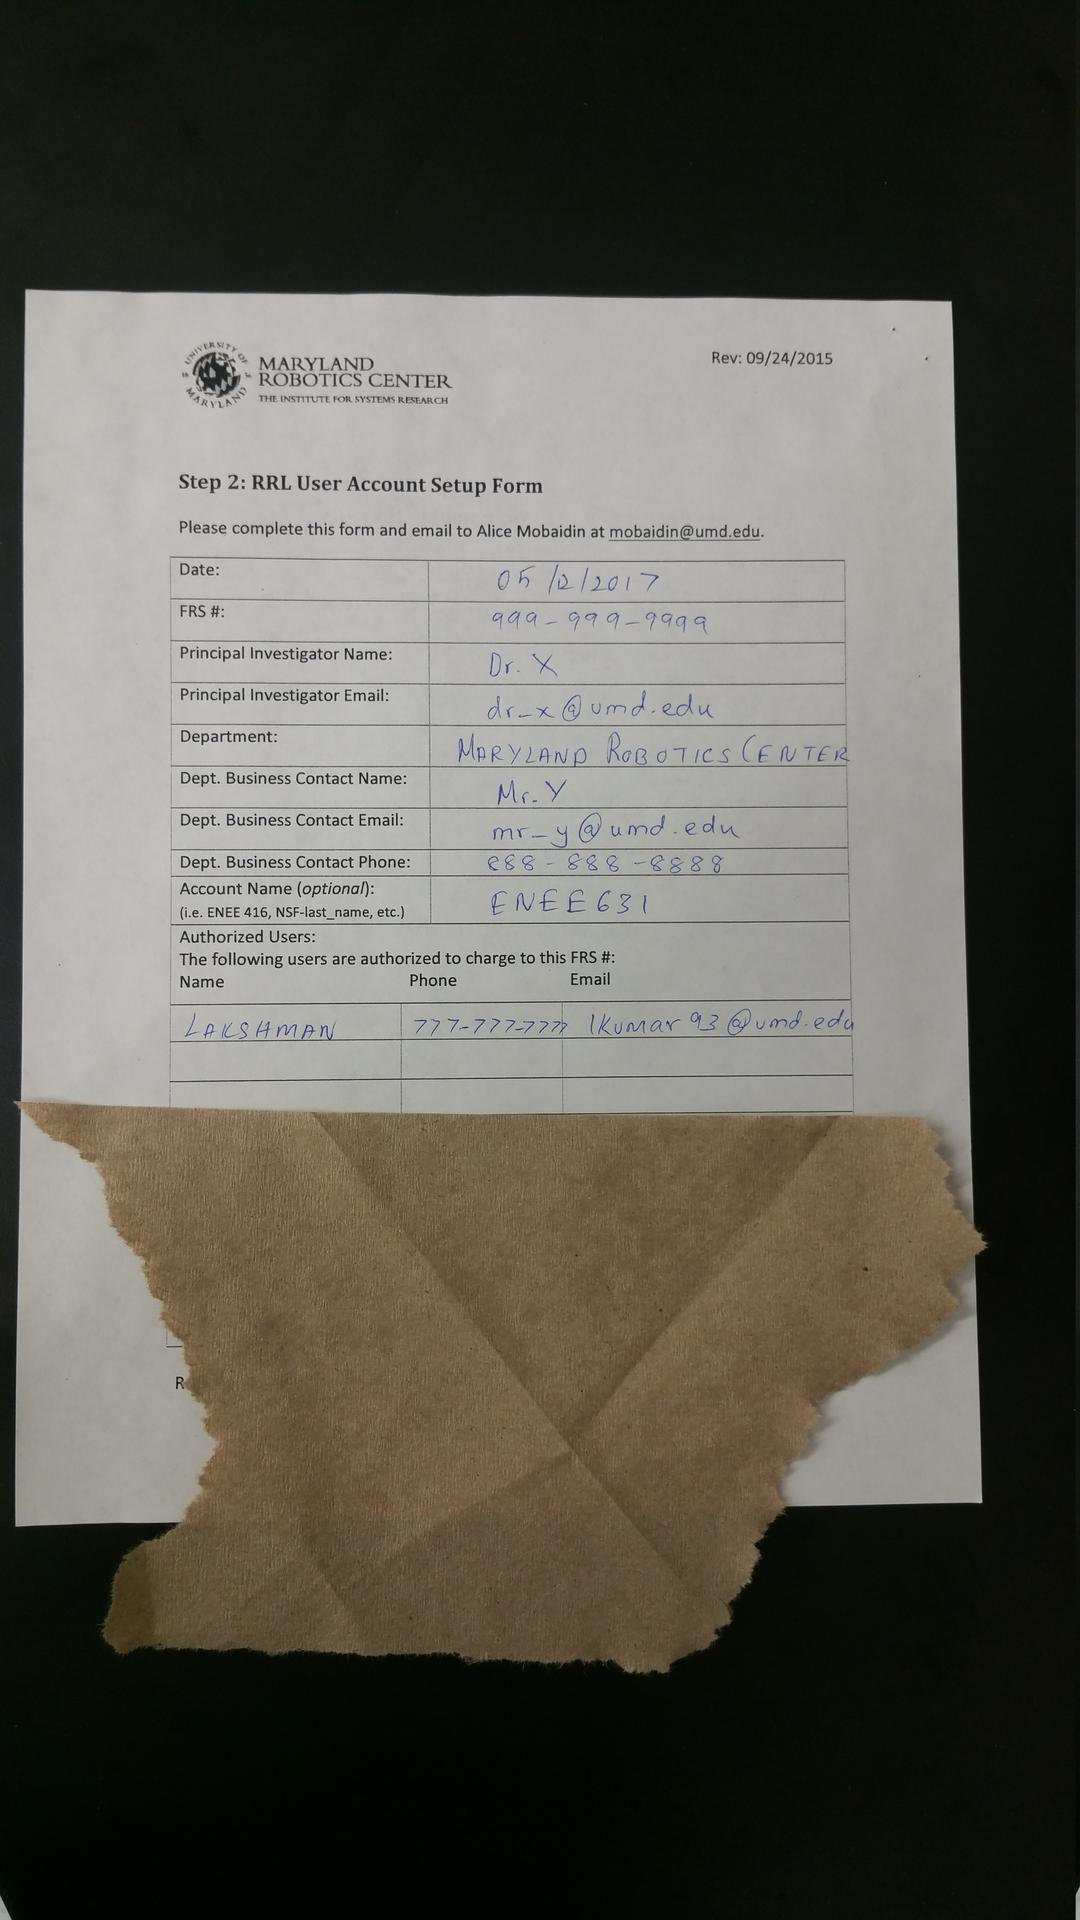
\includegraphics[height=18cm ]{Figures/scanned_image}
	%	\decoRule
	\caption[ScannedImage]{Scanned Image}
	\label{fig:ScannedImage}
\end{figure}

\pagebreak
All the techniques involved in extracting filled text from the scanned image and overlaying it on top of the reference document are briefly explained below. \\

\subsection{Image Alignment}

\keyword{ORB feature detector} (\cite{Reference3}) is an effective replacement to \keyword{SIFT} (\cite{Reference8}) and \keyword{SURF} (\cite{Reference9}) in terms of computation cost. It is basically a rotational invariant version of \keyword{FAST} keypoint detector (\cite{Reference12}) and \keyword{BRIEF} keypoint descriptor (\cite{Reference13}).ORB features are computed in both the reference document and the scanned image using \keyword{OpenCV's feature detection API} . These features are then matched between the reference document and scanned image using \keyword{Brute Force Hamming} technique with \keyword{KNN} (\cite{Reference15}), the rest of features are weeded out. These features are further filtered on whether they satisfy the ratio test and the symmetry test. As per the ratio test, matching features, for which the ratio of the nearest neighbor distance to the second nearest neighbor distance is greater than 0.8, are rejected to extract good matches. As per the symmetry test, good matches that correspond from reference image to scanned image and vice versa should be the same or else they are eliminated. Hence better matches can be extracted. It is also made sure that there are at least 500 matches that satisfy both tests between the two images. Hence the number of ORB features are iteratively increased until this constraint is satisfied. \\ \\
The better matches computed in both the reference document and scanned document are shown below. \\ \\ 
\begin{figure}[th]
	\centering
	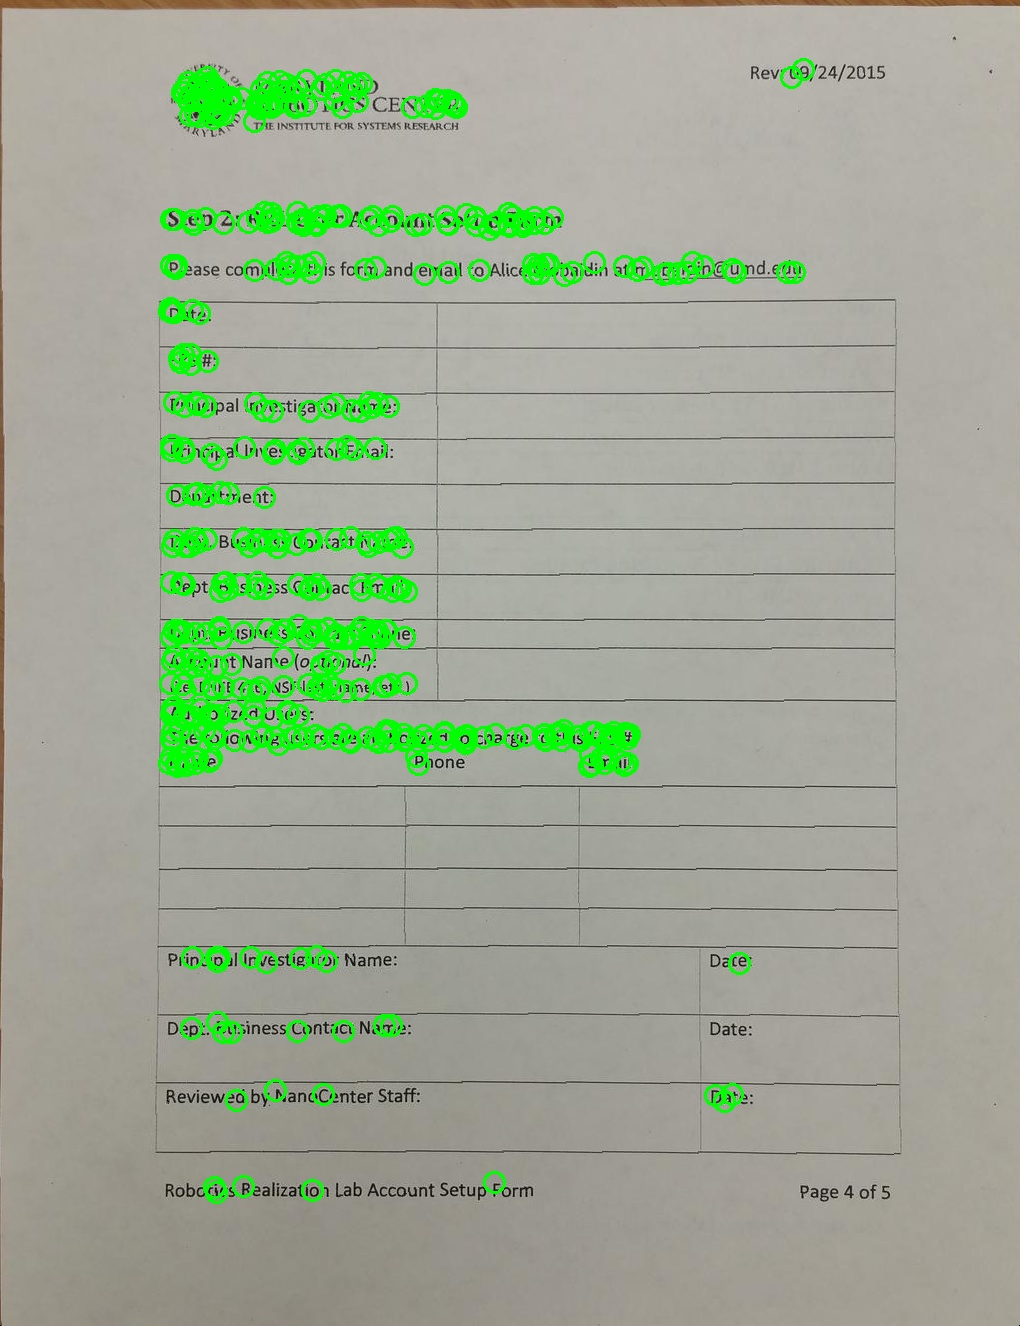
\includegraphics[height=11cm ]{Figures/orb_reference_image}
	%	\decoRule
	\caption[Matching Orb Features in Reference Document]{Matching Orb Features in Reference Document.}
	\label{fig:ReferenceDocumentORBFeatures}
\end{figure}

\pagebreak
\begin{figure}[th]
	\centering
	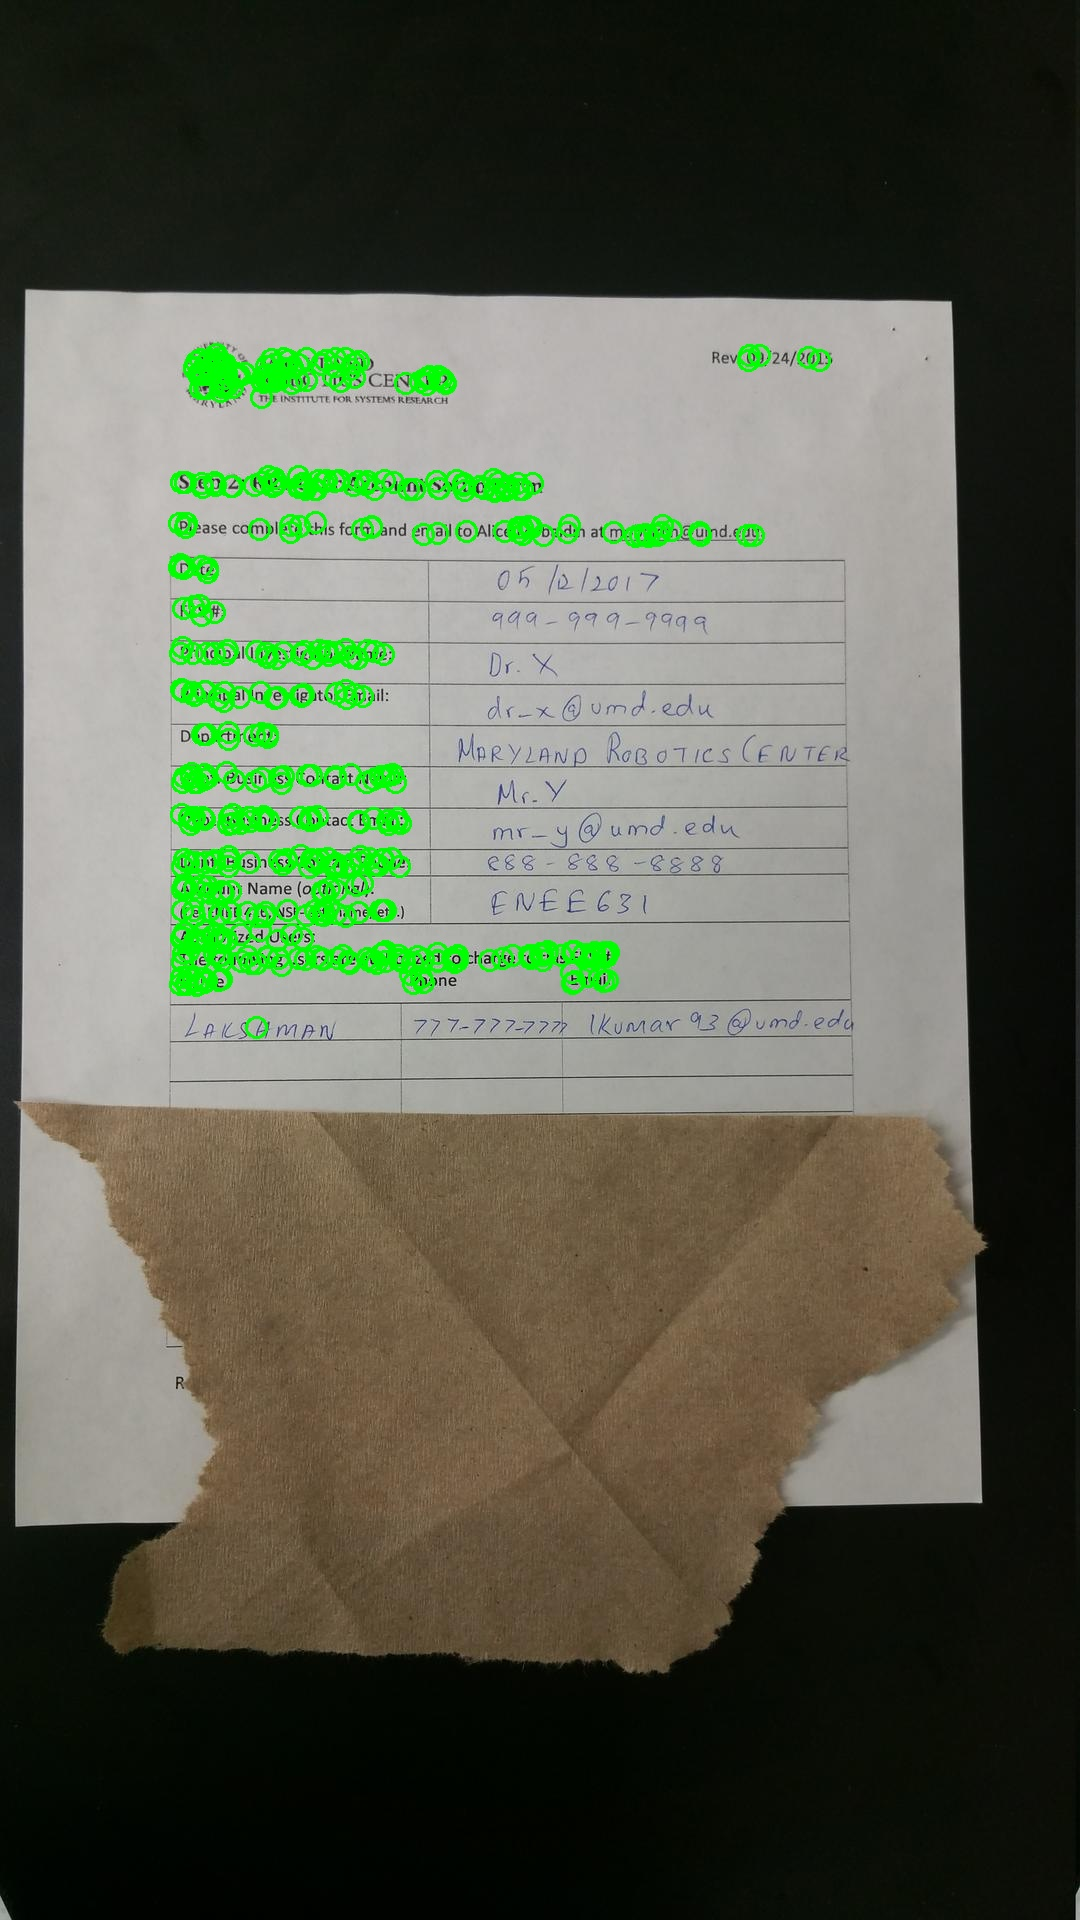
\includegraphics[height=18cm ]{Figures/orb_scanned_image}
	%	\decoRule
	\caption[Matching Orb Features in Scanned Image]{Matching Orb Features in Scanned image.}
	\label{fig:ScannedImageORBFeatures}
\end{figure}

\pagebreak

 In order to obtain the perspective transform linking the two images, 4 matches are required. The best 4 matches can be computed using \keyword{RANSAC} (\cite{Reference11}) . RANSAC is an iterative method to remove outliers. RANSAC initially randomly chooses 4 non-identical matches from the set of better matches and computes the perspective transform between these 4 matches of both the images. The matching features in the scanned image are then warped by the computed perspective transform and checked to see if the euclidean distance between the warped feature and the matching feature in the reference document is less than a certain threshold, which was experimentally determined to be 0.175 . If so, that particular feature is considered to be matching. This process is repeated for all the better matches and for a certain number of iterations, in this case, 50000. The perspective transform that has the most number of matching points is considered to be the best and this is used to warp the scanned image to align with the reference document. \\ \\
 The best four matches are shown below \\ \\ 
 
\begin{figure}[th]
	\centering
	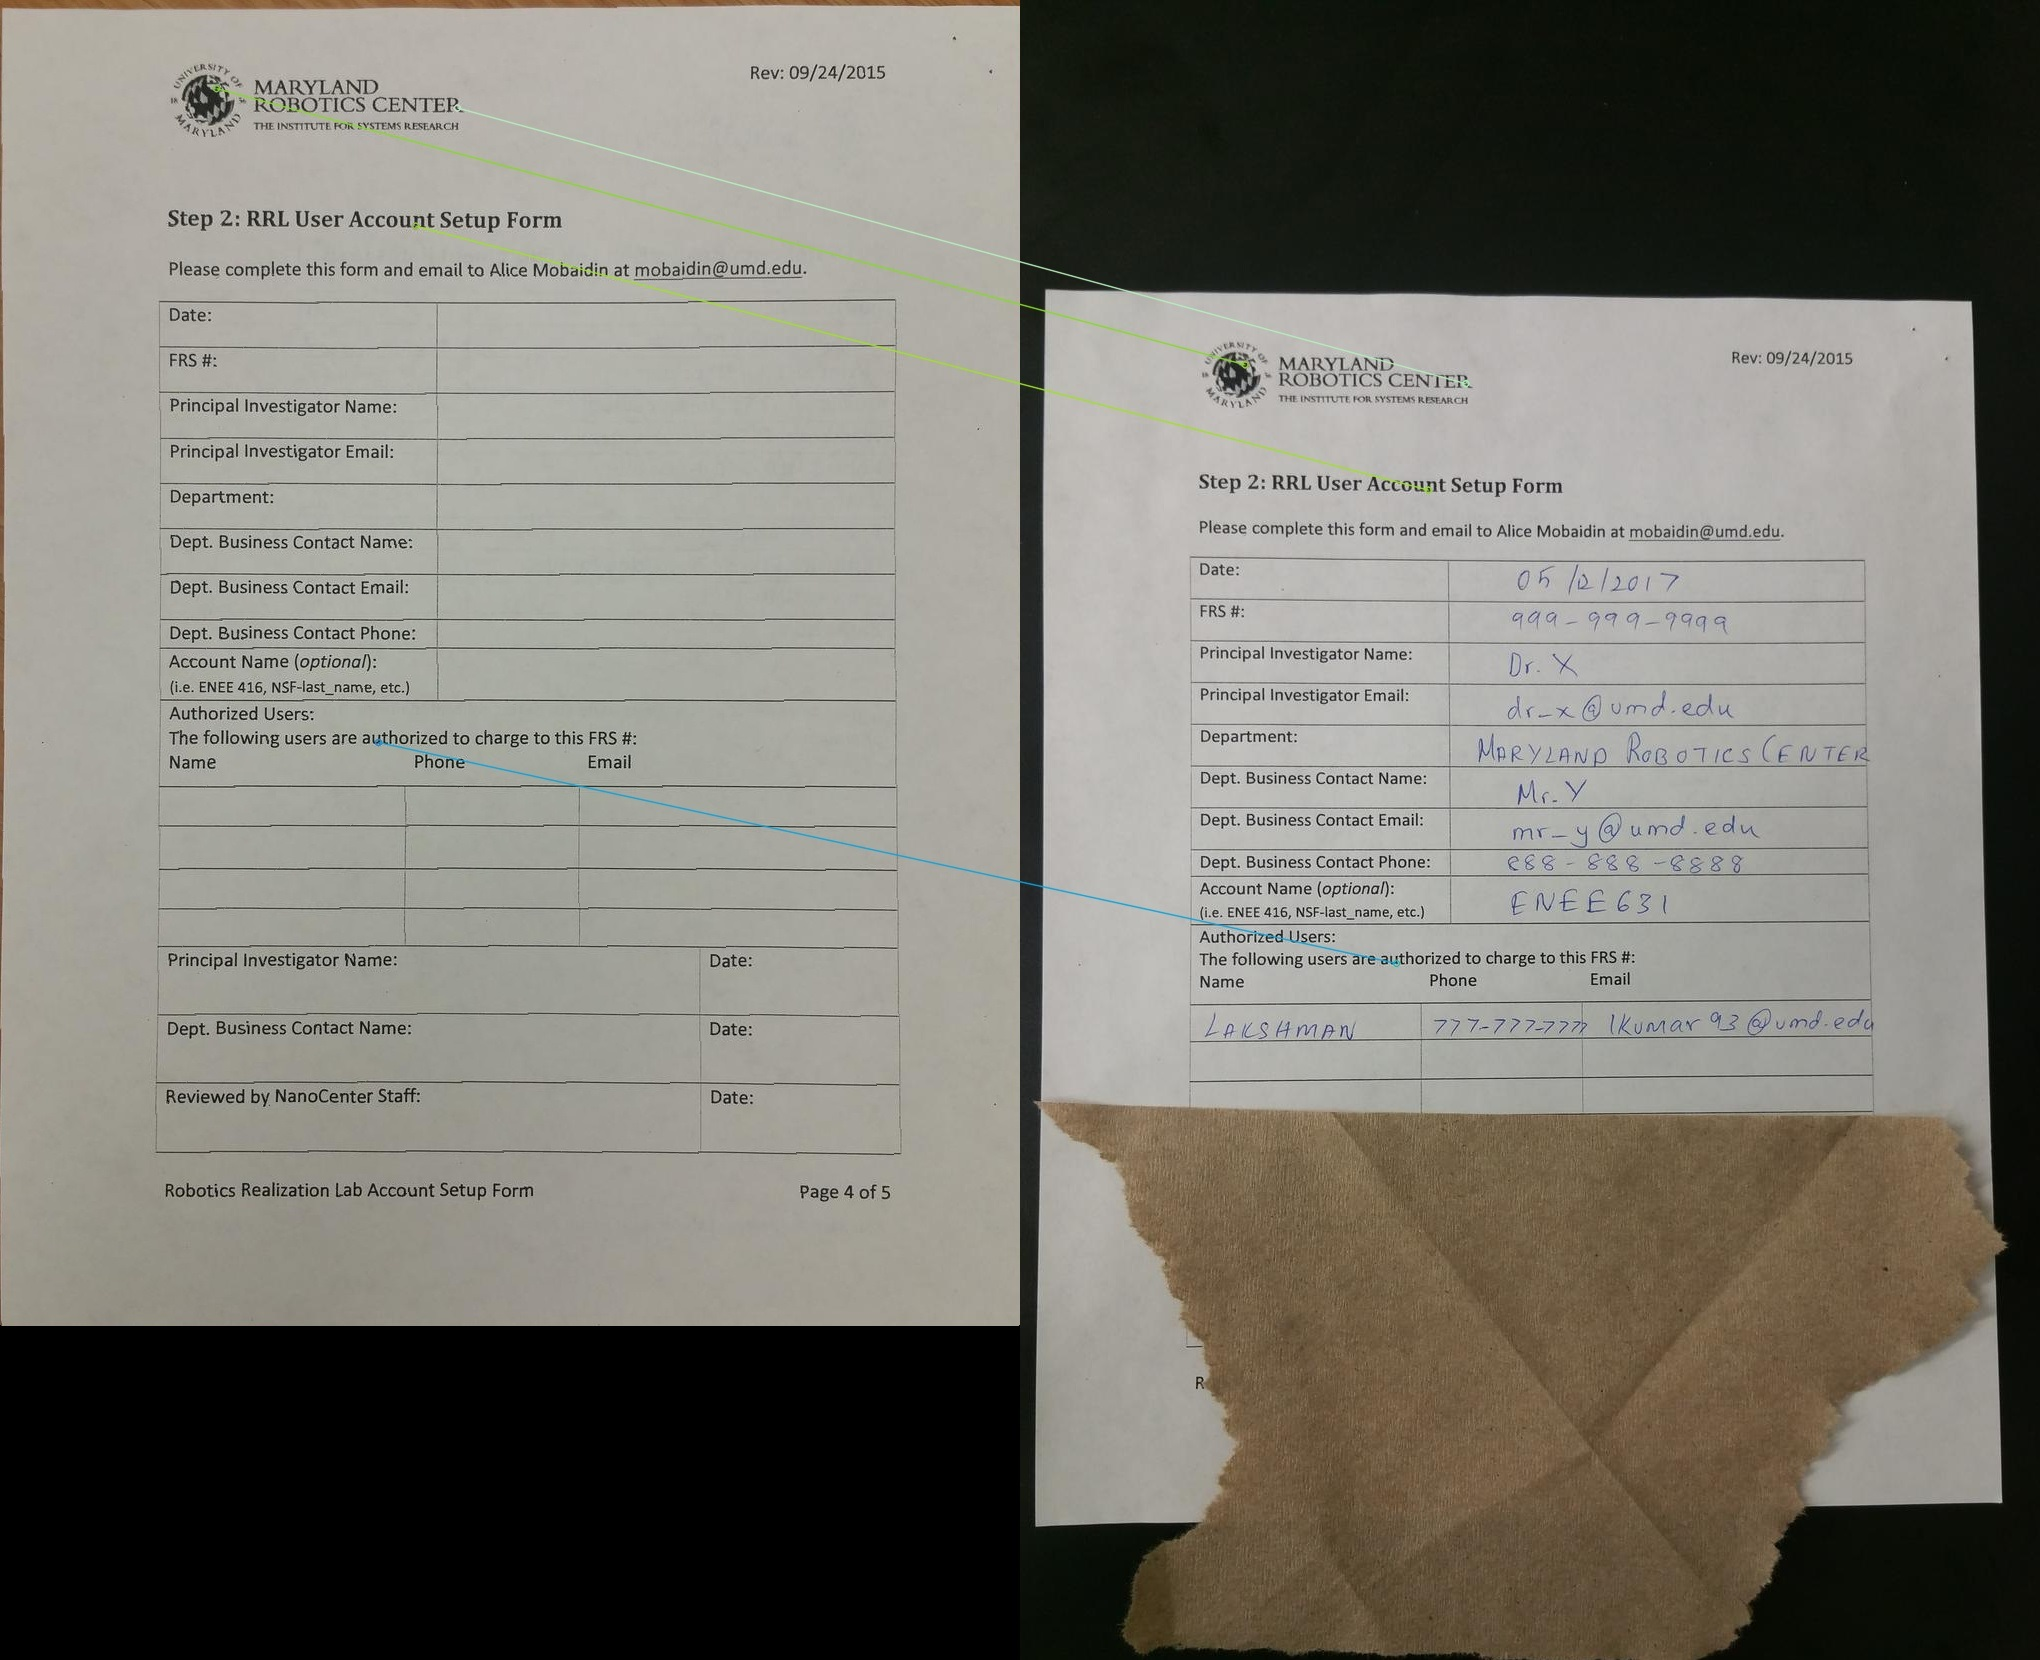
\includegraphics[height=13cm ]{Figures/best_four_matches_ransac}
%	\decoRule
	\caption[Best Matches]{Best Matches.}
	\label{fig:BestMatches}
\end{figure}
\pagebreak

 The aligned version of scanned document is shown below \\ \\ 
 
\begin{figure}[th]
	\centering
	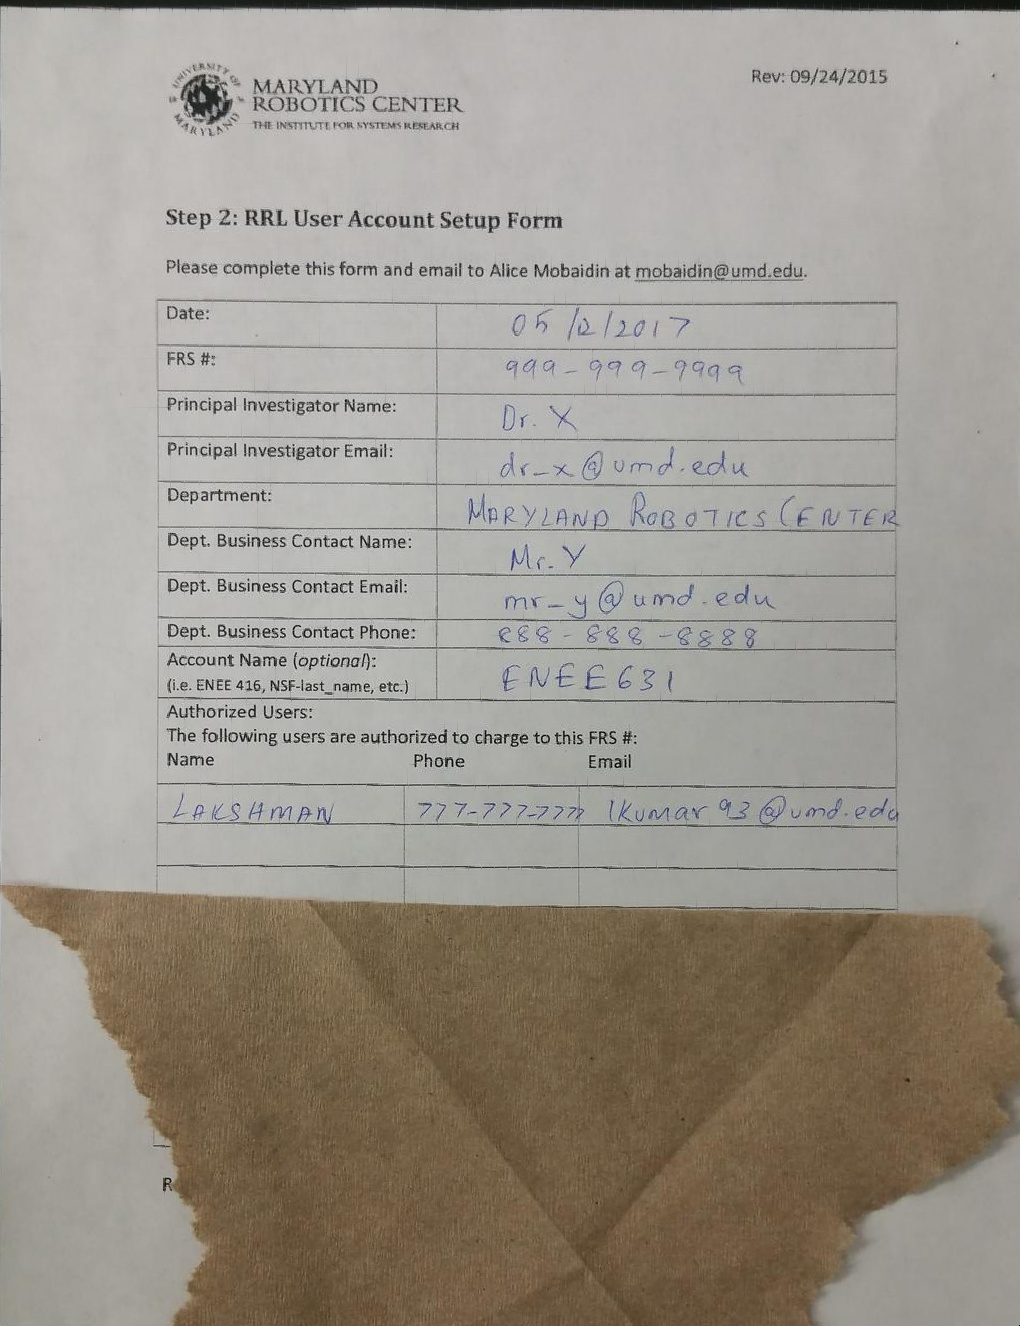
\includegraphics[height=18cm ]{Figures/warped_scanned_image}
	%	\decoRule
	\caption[Warped Scanned Document]{Warped Scanned Document.}
	\label{fig:WarpedFilledDocument}
\end{figure}
\pagebreak


\subsection{Background Subtraction}

Background Subtraction is done in order to extract the filled text from scanned document. In order to do that , both the reference document and the scanned document are converted to grayscale and then sharpened to boost its edges. The sharpened images are then further adaptively thresholded to convert them to a binary image.
\\
\\
The adaptively thresholded images are shown below.
\\
\\
\begin{figure}[th]
	\centering
	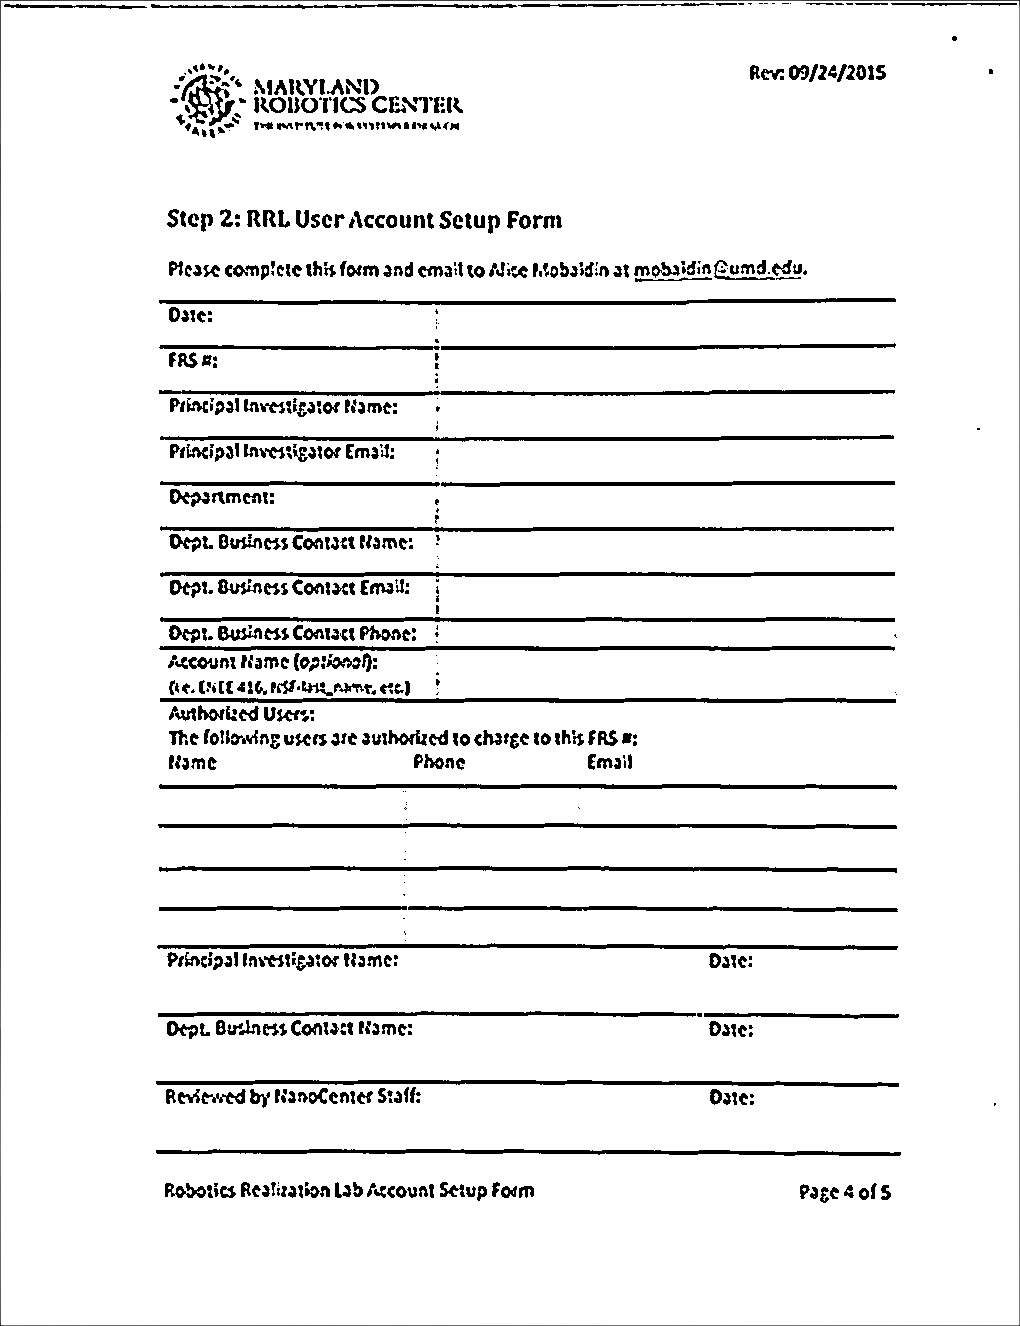
\includegraphics[height=15cm ]{Figures/thresholded_reference_image}
	%	\decoRule
	\caption[Thresholded Reference Document]{Thresholded Reference Document.}
	\label{fig:ThresholdedReferenceDocument}
\end{figure}	

\pagebreak

\begin{figure}[th]
	\centering
	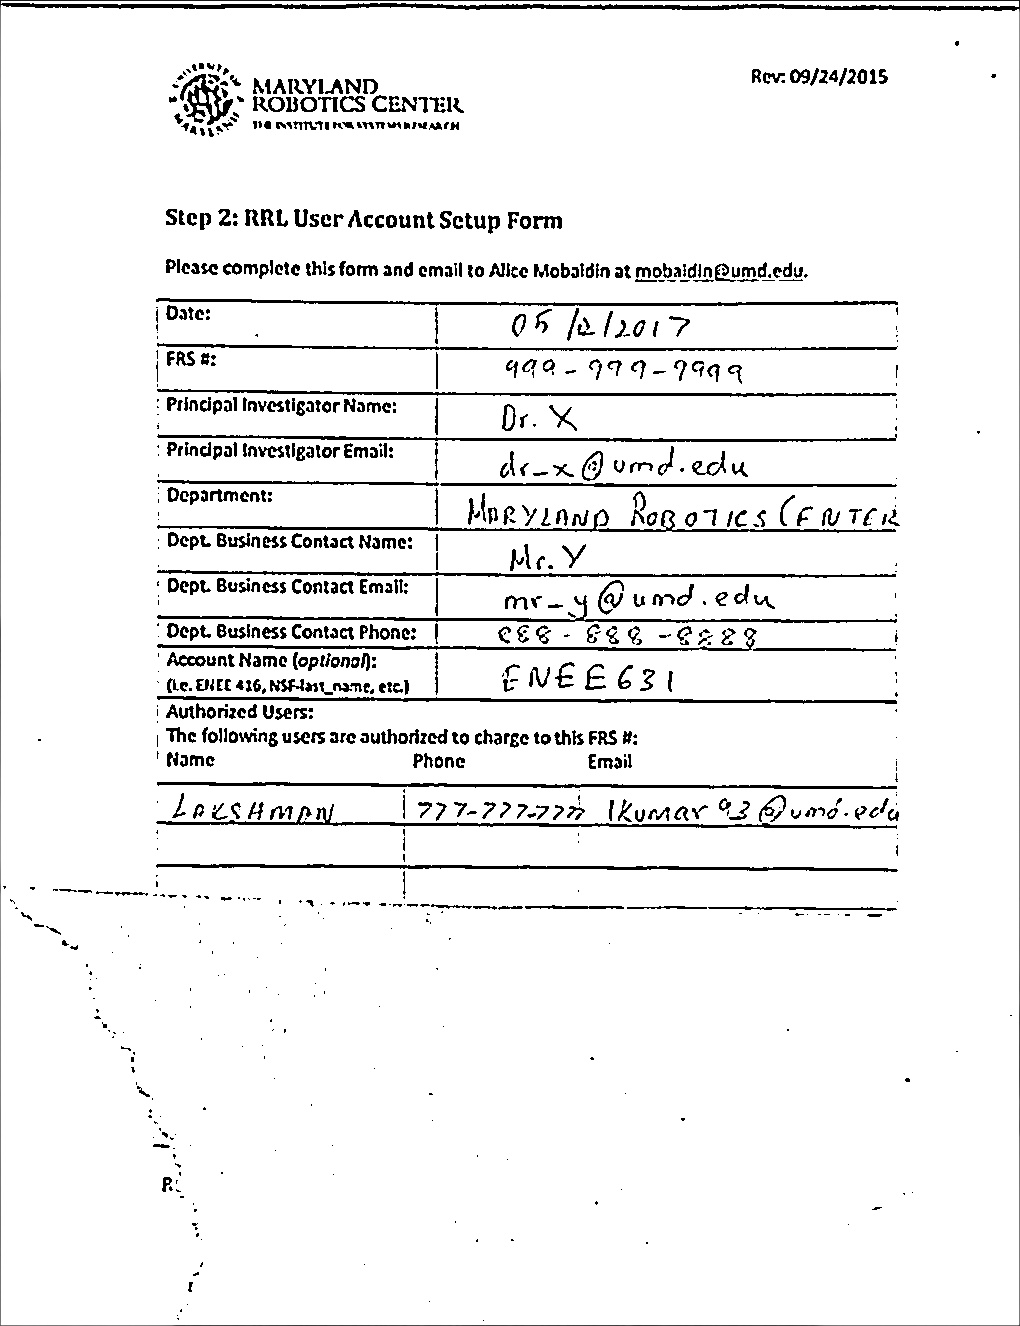
\includegraphics[height=18cm ]{Figures/thresholded_scanned_image}
	%	\decoRule
	\caption[Thresholded Scanned Document]{Thresholded Scanned Document.}
	\label{fig:ThresholdedScannedDocument}
\end{figure}

\pagebreak

Based on the values in both the thresholded images, the additional content in the scanned document is extracted from the reference document . The extracted foreground is then filtered a bit by dilation and median filtering. It can be seen from the image below that almost the entire filled content has been extracted. However, there might be some additional residue due to minute differences in alignment either because of Bilinear Interpolation or lesser number of iterations in RANSAC. \\ \\

\begin{figure}[th]
	\centering
	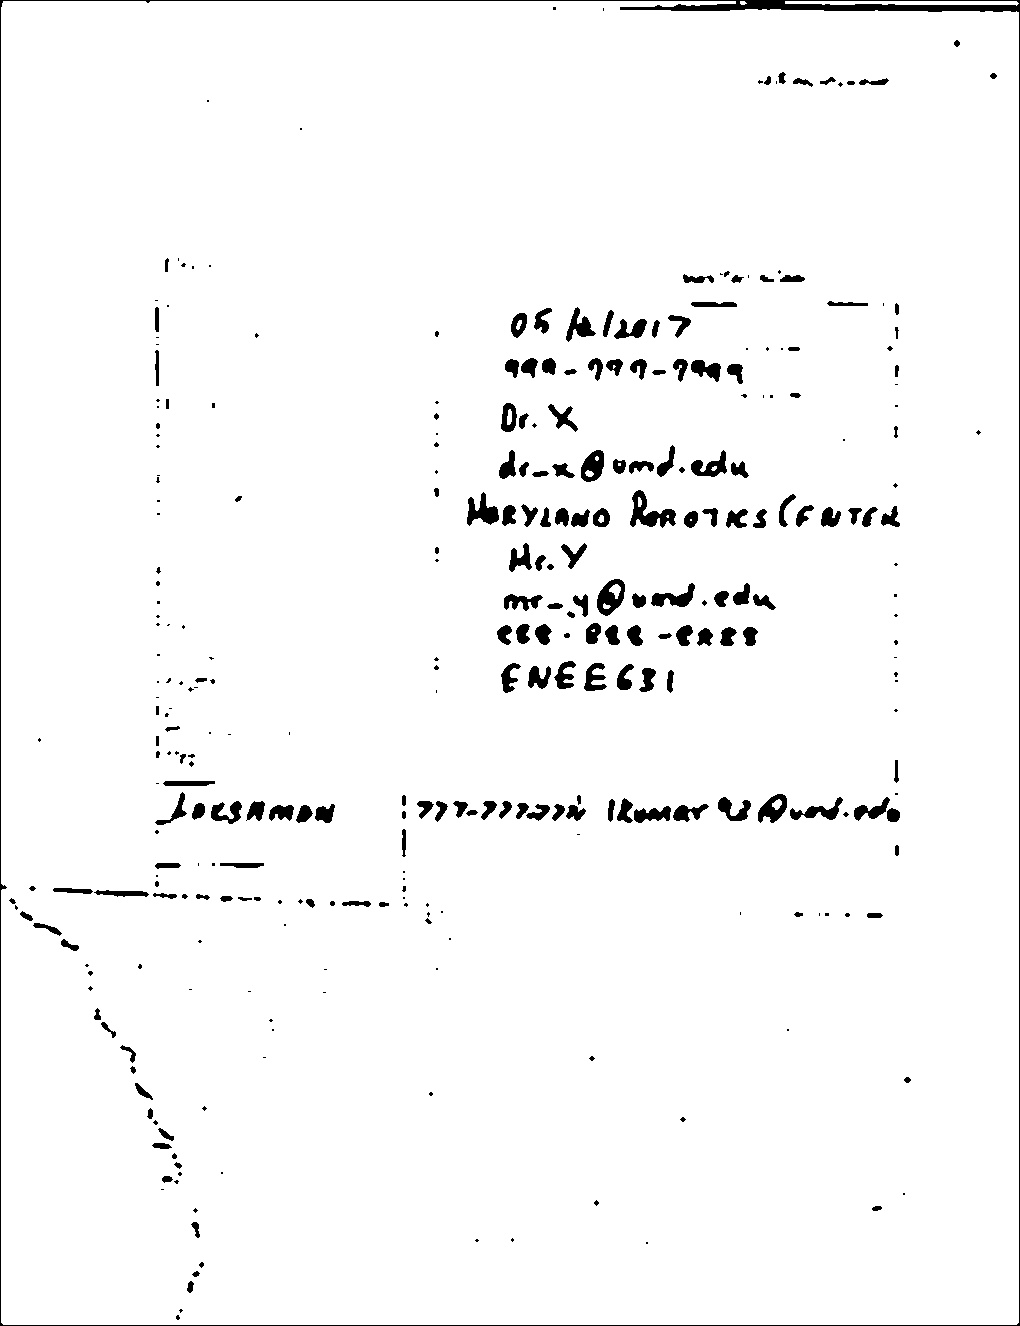
\includegraphics[height=18cm ]{Figures/background_subtraction}
	%	\decoRule
	\caption[Background Subtraction]{Background Subtraction.}
	\label{fig:BackgroundSubtraction}
\end{figure}
\pagebreak
\subsection{Foreground Addition}

Based on the extracted foreground, pixels in the scanned image are overlaid on top of the reference document. From the resultant images, it can be observed that most of the content is properly overlaid, however, there are some noises and artifacts due to border effects, minute differences in alignment, adaptive thresholding parameters and edges of obstructions in the image of scanned document. 
\\
\\
The binary version of the restored image is shown below. \\ 

\begin{figure}[th]
	\centering
	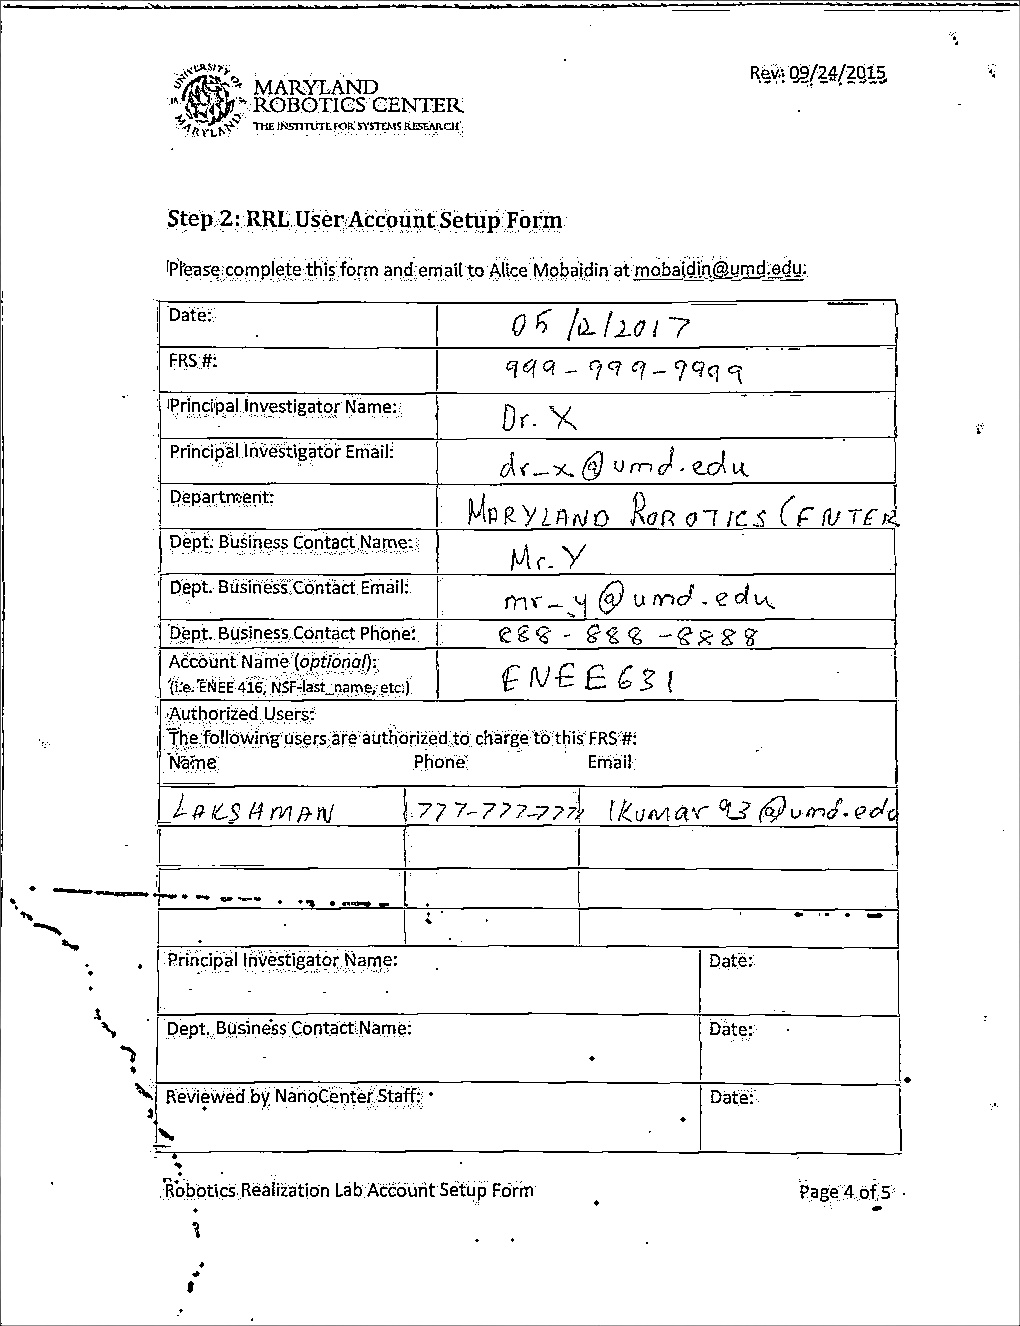
\includegraphics[height=16cm ]{Figures/thresholded_restored_image}
	%	\decoRule
	\caption[Binary Restored Image]{Binary Restored Image.}
	\label{fig:BinaryRestoredImage}
\end{figure}

\pagebreak

The RGB version of the restored image is shown below. \\  \\

\begin{figure}[th]
	\centering
	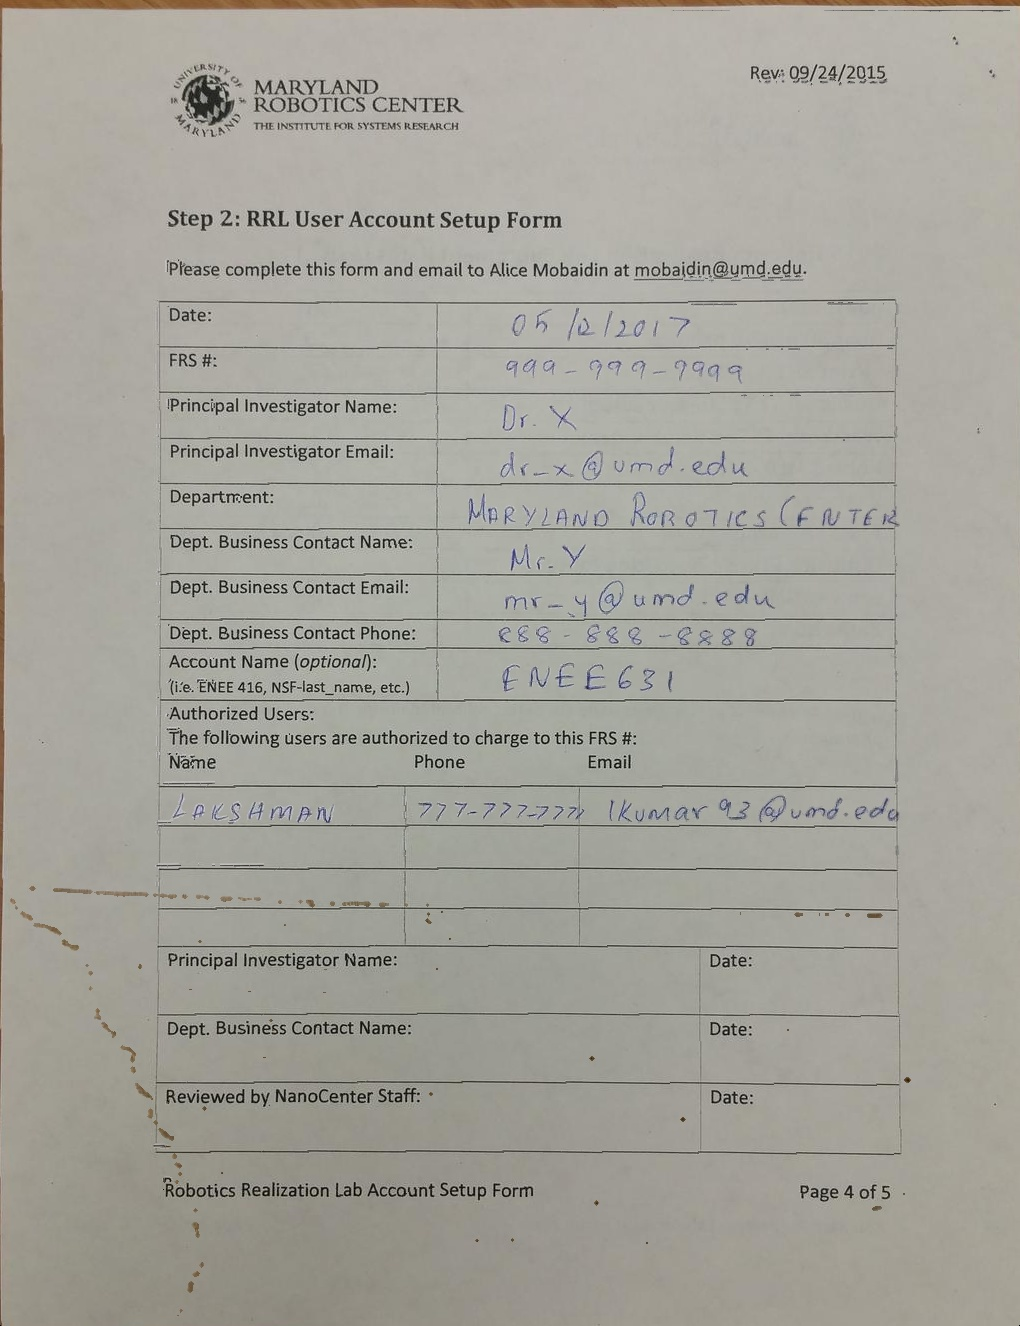
\includegraphics[height=18cm ]{Figures/restored_image}
	%	\decoRule
	\caption[Restored Image]{Restored Image.}
	\label{fig:RestoredImage}
\end{figure}

\pagebreak


%----------------------------------------------------------------------------------------


